\documentclass[../main.tex]{subfiles}
\begin{document}

\section{Pose Estimation of Objects} \label{sec:vision}
In this section, two simple pose estimation methods are outlined to estimate the pose of an object in a scene. The same object is used in both of the methods. In Section \ref{subsec:method2}, a method for pose estimation is described which uses a simulated depth sensor in RobWorks. In Section \ref{subsec:method3}, a method for position estimation by the use of two cameras in RobWorks is described. The two implemented methods are compared in Section \ref{subsec:vision_comparison}.

\subsection{Method 2: Simulated Depth Sensor} \label{subsec:method2}
This pose estimation method uses the simulated depth sensor in RobWorks and computes the object pose in the scene by the use of point clouds \cite{point_cloud_library}. The goal is to estimate a pose that has the minimum sum of distances between the object points and the scene points. The pipeline for the simulated depth sensor method is illustrated in Figure \ref{fig:sds_process}.
\begin{figure}[H]
    \centering
    \noindent\makebox[\textwidth][c]{\subfile{figures/simulated_depth_sensor/sds_process}}
    \caption{Illustration of the pipeline for the simulated depth sensor method.}
    \label{fig:sds_process}
\end{figure}
The pipeline of the simulated depth sensor, shown in Figure \ref{fig:sds_process}, is described further below.
\begin{enumerate}
    \item A point cloud of the scene is loaded from the simulated depth sensor, this is shown in Figure \ref{subfig:sds_initial_scene}.
    \item The point cloud is processed, thus irrelevant information is discarded. An illustration of the processed point cloud and the object point cloud is shown in Figure \ref{subfig:sds_filtered_scene}, where green points are the input point cloud and the red points are the object point cloud.
    \item The object is globally aligned in the scene, which is illustrated in Figure \ref{subfig:sds_after_global}.
    \item The object is locally aligned in the scene, this is illustrated in Figure \ref{subfig:sds_after_local}.
    \item The estimated pose is found.
\end{enumerate}
\begin{figure}[H]
    \centering
    \begin{subfigure}[t]{0.2\textwidth}
        \centering
        \captionsetup{width=.9\textwidth}
        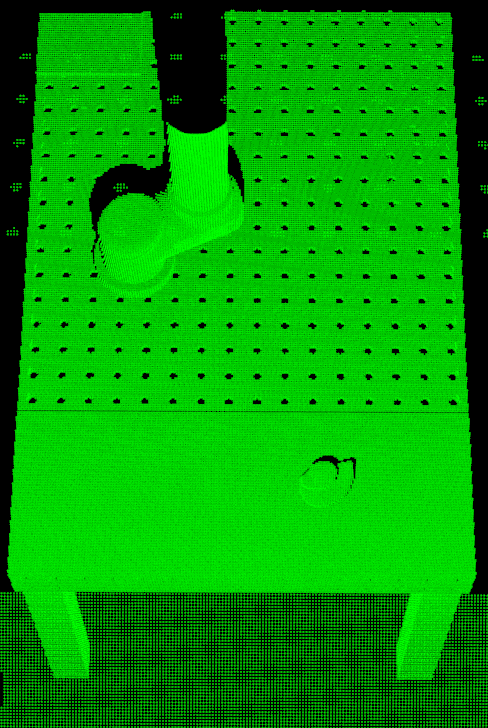
\includegraphics[width=0.9\textwidth]{figures/simulated_depth_sensor/scene_before_preprocessing.png}
        \caption{Input cloud from depth sensor.}
        \label{subfig:sds_initial_scene}
    \end{subfigure}
    \begin{subfigure}[t]{0.2\textwidth}
        \centering
        \captionsetup{width=.9\textwidth}
        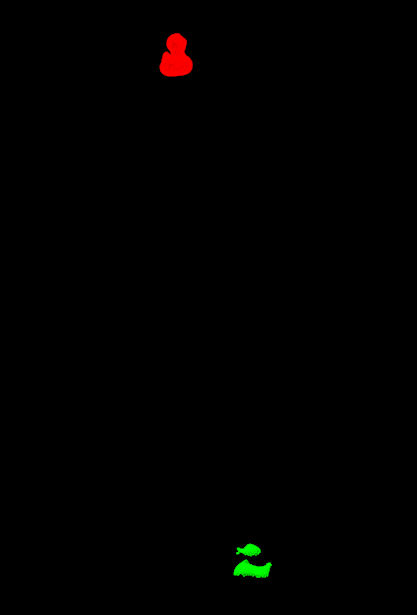
\includegraphics[width=0.9\textwidth]{figures/simulated_depth_sensor/scene_after_preprocessing.png}
        \caption{Processed input cloud.}
        \label{subfig:sds_filtered_scene}
    \end{subfigure}
    \begin{subfigure}[t]{0.2\textwidth}
        \centering
        \captionsetup{width=.9\textwidth}
        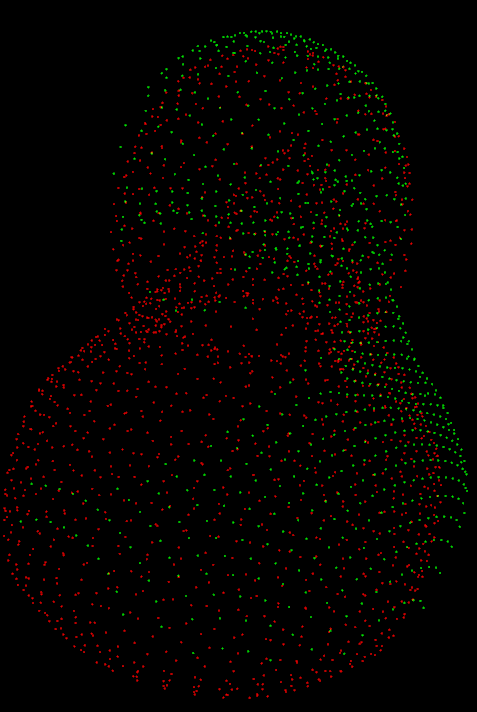
\includegraphics[width=0.9\textwidth]{figures/simulated_depth_sensor/after_global_alignment.png}
        \caption{After global alignment.}
        \label{subfig:sds_after_global}
    \end{subfigure}
    \begin{subfigure}[t]{0.2\textwidth}
        \centering
        \captionsetup{width=.9\textwidth}
        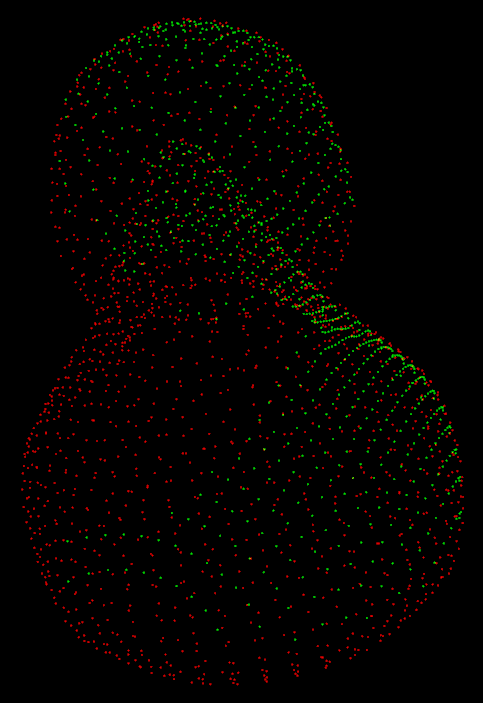
\includegraphics[width=0.9\textwidth]{figures/simulated_depth_sensor/after_local_alignment.png}
        \caption{After local alignment.}
        \label{subfig:sds_after_local}
    \end{subfigure}
    \caption{Example of the simulated depth sensor pipeline. Green points are scene points and red points are object points.}
    \label{fig:sds_pictures}
\end{figure}

\subsubsection{Point Cloud Processing} \label{subsubsec:filter_input}
Before the pose of the object is found the scene is processed, thereby making the alignment of the object in the scene easier both computationally and pose estimation wise. Figure \ref{fig:filter_process} shows the implemented point cloud processing pipeline. 

\begin{figure}[H]
    \centering
    \noindent\makebox[\textwidth][c]{\subfile{figures/simulated_depth_sensor/filter/filter_figure}}
    \caption{Illustration of the point cloud processing pipeline with noise from a normal distribution with a standard deviation of $0.005$. Green points are the input points from the simulated depth sensor, and red points are the true pose of the object.}
    \label{fig:filter_process}
\end{figure}

In Figure \ref{fig:filter_process}a, the scene is loaded from the scanner and noise with a standard deviation of 0.005 is added to the scene. Then, in Figure \ref{fig:filter_process}b, the scene is passed through a spatial filter that removes points outside intervals in $x$, $y$, and $z$. This filtering is based on the scene and the placement of the scanner, thus everything outside of the picking area is removed. Afterwards in Figure \ref{fig:filter_process}c, the scene point cloud is downsampled using a voxelized grid approach with a leaf size of $0.005$ meter. Then in Figure \ref{fig:filter_process}d, the scene is resampled by moving least squares with a polynomial order of $2$ and a sphere search radius of $0.01$ meter. In Figure \ref{fig:filter_process}e, a simple plane segmentation is performed which removes points in the point cloud that support a plane model. The distance, which determines how close a point must be to be considered an inlier of the plane, is set to $0.01$ meter. Lastly in Figure \ref{fig:filter_process}e outliers are removed, by the use of statistics of the whole point cloud to determine which points are too far from the other points. The implemented outlier removal looks at $100$ neighbors for each point, and if the distance is larger than $0.1$ of the mean distance to the query point the point will be removed. After the filter process, the final input point cloud is passed on to the global alignment block, which is described below.

\subsubsection{Global Alignment} \label{subsubsec:global_alignment}
This method finds the pose of a 3D object, which brings the object into optimal alignment in a given 3D scene. The pipeline of global alignment is illustrated in Figure \ref{fig:global_process}.
\begin{figure}[H]
    \centering
    \noindent\makebox[\textwidth][c]{\subfile{figures/simulated_depth_sensor/global/global_figure}}
    \caption{Illustration of the global alignment pipeline.}
    \label{fig:global_process}
\end{figure}
\textbf{Estimate surface normals:}\\
The surface normal is computed as the normal on the plane fitted to the points within a certain radius. The surface normals are used for computing the feature descriptors used for matching between the object and scene. In Figure \ref{fig:sds_normals}, the estimated surface normals with different radii are shown. The radius must be larger than the voxel grid leaf size, e. g. in Figure \ref{subfig:sds_normals_0.001} no surface normals are found when the radius is $0.001$ meter, however the radius must not be too big either as illustrated in Figure \ref{subfig:sds_normals_0.1}. Through several observations and experiments the radius was chosen to $0.01$ meter.
\begin{figure}[H]
    \centering
    \begin{subfigure}[t]{0.19\textwidth}
        \centering
        \captionsetup{width=0.85\textwidth}
        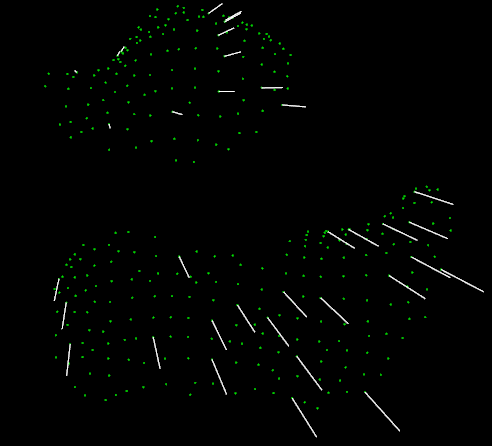
\includegraphics[width=0.85\textwidth]{figures/simulated_depth_sensor/global/normals_1.png}
        \caption{Estimated surface normals with a radius of $0.1$ meter.}
        \label{subfig:sds_normals_0.1}
    \end{subfigure}
    \begin{subfigure}[t]{0.17\textwidth}
        \centering
        \captionsetup{width=0.85\textwidth}
        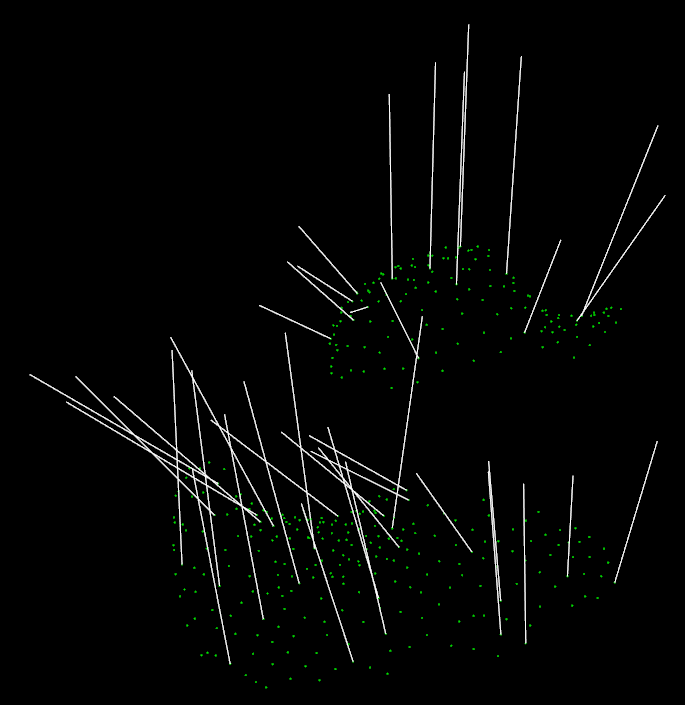
\includegraphics[width=0.85\textwidth]{figures/simulated_depth_sensor/global/normals_05.png}
        \caption{Estimated surface normals with a radius of $0.05$ meter.}
        \label{subfig:sds_normals_0.05}
    \end{subfigure}
    \begin{subfigure}[t]{0.18\textwidth}
        \centering
        \captionsetup{width=.85\textwidth}
        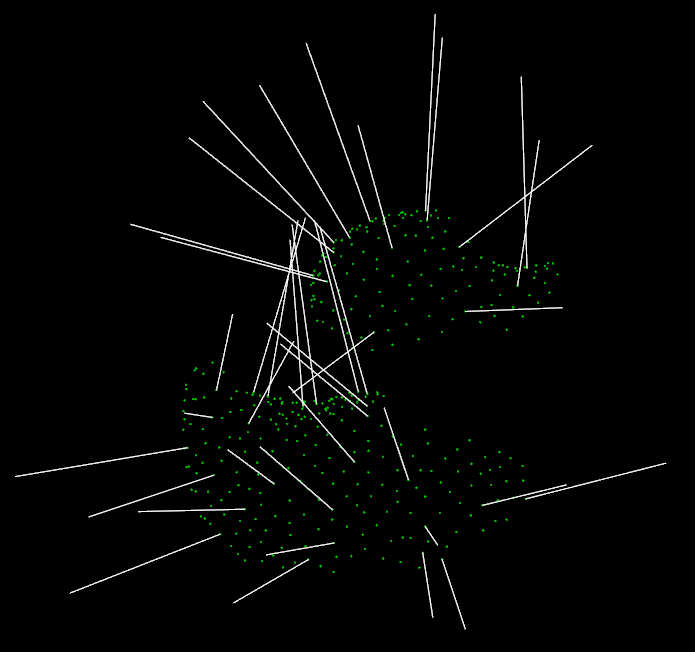
\includegraphics[width=0.85\textwidth]{figures/simulated_depth_sensor/global/normals_01.png}
        \caption{Estimated surface normals with a radius of $0.01$ meter.}
        \label{subfig:sds_normals_0.01}
    \end{subfigure}
    \begin{subfigure}[t]{0.17\textwidth}
        \centering
        \captionsetup{width=0.85\textwidth}
        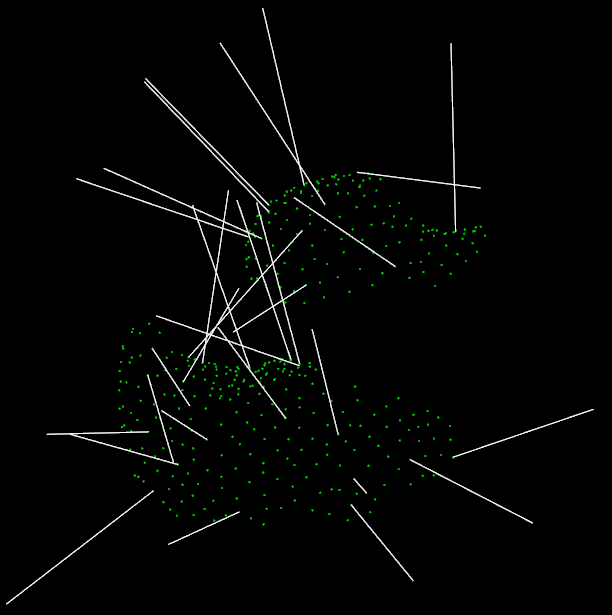
\includegraphics[width=0.85\textwidth]{figures/simulated_depth_sensor/global/normals_005.png}
        \caption{Estimated surface normals with a radius of $0.005$ meter.}
        \label{subfig:sds_normals_0.005}
    \end{subfigure}
    \begin{subfigure}[t]{0.19\textwidth}
        \centering
        \captionsetup{width=0.825\textwidth}
        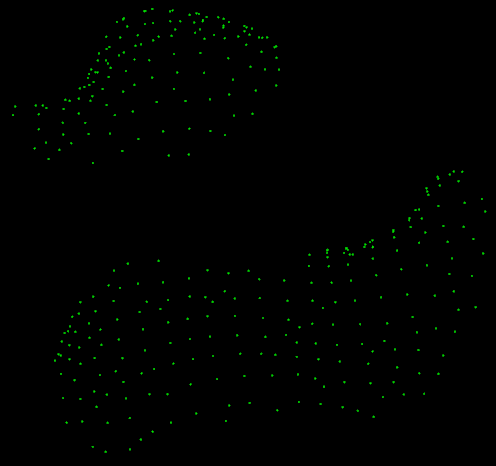
\includegraphics[width=0.825\textwidth]{figures/simulated_depth_sensor/global/normals_001.png}
        \caption{Estimated surface normals with a radius of $0.001$ meter.}
        \label{subfig:sds_normals_0.001}
    \end{subfigure}
    \caption{Illustration of estimated surface normals of the scene with different radii after filtering.}
    \label{fig:sds_normals}
\end{figure}
\textbf{Estimate Features Descriptor:}\\
A very important element in pose estimation is to find the correct corresponding points between the object and scene, thus to match points a local feature descriptor is used. The used feature descriptor method is Fast Point Feature Histogram, FPFH, which is introduced in \cite{fpfh} and also used in \cite{buch2013pose}. Based on the results in \cite{fpfh} and \cite{buch2013pose} it was chosen to use FPFH. FPFH constructs a 33-dimensional histogram by:
\begin{enumerate}
    \item Finding all oriented points in a spherical neighborhood of a certain radius around each point.
    \item Computing relative angles using the estimated surface normals from before, and the direction vector from the source point to each neighbor point.
\end{enumerate}
The radius used for the neighbor search must be bigger or equal to the radius used for estimating the surface normals. The implemented radius is set to $0.01$ meter, which was found to be reasonable. Figure \ref{fig:feature_matching} shows the feature matches between the input point cloud, the green points, and the object point cloud, the red points.
\begin{figure}[H]
    \centering
    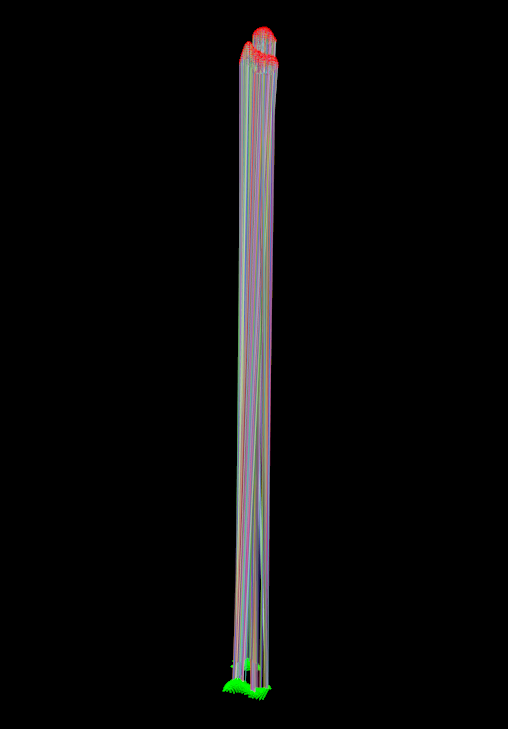
\includegraphics[width=0.9\textwidth]{figures/simulated_depth_sensor/global/feature_matching.png}
    \caption{Illustrations of the feature matching between the input point cloud, the green points, and the object, the red points. The image is rotated 90 degrees to the right.}
    \label{fig:feature_matching}
\end{figure}
\textbf{Random Sample Consensus:}\\
To estimate the transformation, T, which transforms the object points, p, into the scene points, q, the Kabsch algorithm \cite{kabsch_algorithm} is used to solve the equation $q\ =\ T \cdot p$. However, because of the uncertainty of whether the found correspondences are the true correspondences between the object and the scene a RANdom SAmple Consensus \cite{RANSAC}, RANSAC, method is implemented. The implemented RANSAC method is based on the paper \cite{buch2013pose}, which outlines a simple and robust estimation algorithm that performs 15 times faster than standard RANSAC. The steps of the algorithm are:
\begin{enumerate}
    \item \label{ransac:step1} Find 3 random object points and their correspondences in the scene, by nearest neighbor matching of the feature descriptors.
    \item Calculate the ratio between the edge lengths of the polygons formed by the 3 points on both the object and the scene. If the similarity is below a certain threshold go to step \ref{ransac:step1}.
    \item Estimate the transformation using the 3 point correspondences from step \ref{ransac:step1}, and apply it to the object.
    \item Save the transformation if the number of inliers is the highest so far and above the required number of inlier points.
    \item Stop the algorithm after a certain number of iterations otherwise go to step \ref{ransac:step1}.
\end{enumerate}
The implemented RANSAC method samples 3 points in step \ref{ransac:step1}, which is the minimum requirement for 6 Degrees of Freedom, DoF. The inlier fraction of inlier points required for accepting a transformation is set to $0.05$ as in \cite{buch2013pose}, this was observed to have the best performance. The similarity between the polygon edges is set to $0.9$, thus creating a quite strict rejector but making the execution time of the RANSAC much faster. The maximum distance between two corresponding points in object and scene is set to $0.0075$ meter, which is based on the voxel grid leaf size and experience. The maximum number of iterations, k, given a desired success probability, $p\ =0.99$, an expected inlier fraction, $w\ =0.05$, and sample points, $n\ =3$ is \cite{RANSAC}:
\begin{equation}
    Iterations\ = \frac{log(1-p)}{log(1-w^n)} = \frac{log(1-0.99)}{log(1-0.05^3)} = 36839
\end{equation}
However, to ensure a more precise pose estimation the iterations are set to 80000.

\subsubsection{Local Alignment} \label{subsubsec:local_alignment}
The local alignment pose estimation finds the optimal alignment of two 3D models, which are almost aligned. The implemented local alignment is based on the algorithm Iterative Closest Point, ICP, which is introduced in \cite{alignment}. The steps implemented are:
\begin{enumerate}
    \item \label{local:step1} Find nearest neighbors between the transformed object and the scene, and threshold neighbors by euclidean distance.
    \item Estimate the transformation using the neighbor correspondences.
    \item Apply the transformation to the object points.
    \item Stop the algorithm after a certain number of iterations otherwise go to step \ref{local:step1}.
\end{enumerate}
The implemented ICP method is set to run for $500$ iterations, which deemed acceptable in execution time versus pose estimation precision. Furthermore, the euclidean distance threshold for accepting neighbors was set to $0.0001$. Thereby, ensuring the method not to use point correspondences which are most likely not true correspondences.

\subsubsection{Evaluation of the Method} \label{subsubsec:eval_method2}
To evaluate the method 30 random positions with a random rotation around the z-axis are generated, and noise from a normal distribution is added to the simulated depth sensor input point cloud. The real transformation is generated from RobWorks, which is described as $T_{Table}^{Real pose}$. However, the estimated transformation is described as $T_{Scanner}^{Estimated pose}$, thus to compare the two transformations the following equation is used: 
\begin{equation}
\begin{split}
    T_{World}^{Table} \cdot T_{Table}^{Real\ pose} = T_{World}^{Scanner} \cdot T_{Scanner}^{Estimated\ pose} \Rightarrow \\
    T_{Table}^{Real\ pose} = \left ( T_{World}^{Table} \right )^{-1} \cdot T_{World}^{Scanner} \cdot T_{Scanner}^{Estimated\ pose}
\end{split}
\end{equation}
Two illustrations of the random transformation of the object and the found alignment is shown in Figure \ref{fig:random_positions}.
\begin{figure}[H]
    \centering
    \begin{subfigure}[t]{0.4\textwidth}
        \centering
        \captionsetup{width=0.85\textwidth}
        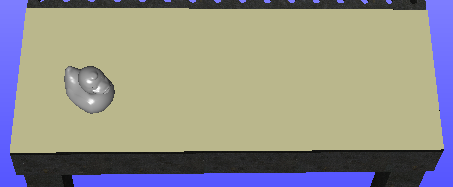
\includegraphics[width=0.85\textwidth]{figures/simulated_depth_sensor/analysis_ex1.png}
        \caption{Random transformation of the object.}
        \label{subfig:rand_pos1}
    \end{subfigure}
    \begin{subfigure}[t]{0.4\textwidth}
        \centering
        \captionsetup{width=0.85\textwidth}
        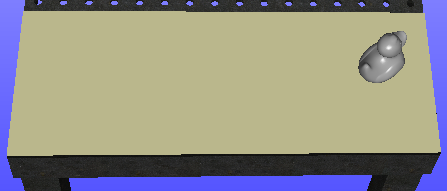
\includegraphics[width=0.85\textwidth]{figures/simulated_depth_sensor/analysis_ex2.png}
        \caption{Random transformation of the object}
        \label{subfig:rand_pos2}
    \end{subfigure}
    
    \begin{subfigure}[t]{0.4\textwidth}
        \centering
        \captionsetup{width=.85\textwidth}
        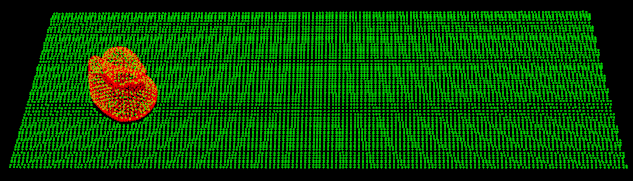
\includegraphics[width=0.85\textwidth]{figures/simulated_depth_sensor/analysis_pcl_ex1.png}
        \caption{Alignment of the object, the red points, in the input cloud, the green points, from Figure \ref{subfig:rand_pos1}.}
        \label{subfig:align_pos1}
    \end{subfigure}
    \begin{subfigure}[t]{0.4\textwidth}
        \centering
        \captionsetup{width=0.85\textwidth}
        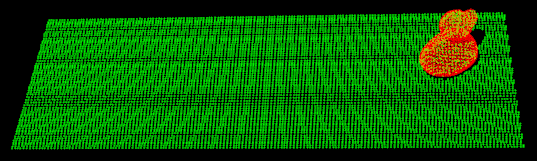
\includegraphics[width=0.85\textwidth]{figures/simulated_depth_sensor/analysis_pcl_ex2.png}
        \caption{Alignment of the object, the red points, in the input cloud, the green points, from Figure \ref{subfig:rand_pos2}.}
        \label{subfig:align_pos2}
    \end{subfigure}
    \caption{Illustration of two of the random transformations of the object, which are used for the evaluation of method 2.}
    \label{fig:random_positions}
\end{figure}
The method is evaluated on three parameters: execution time, difference in angle between real transformation and estimated transformation and the euclidean distance between the real transformation and the estimated transformation. To compare the rotations the intrinsic notion of distance, which is introduced in \cite{compare_rotations}, is used. In Figure \ref{fig:method3_noise_analysis} the results from the evaluation are shown. 
\begin{figure}[H]
    \centering    
    \noindent\makebox[\textwidth]{%
    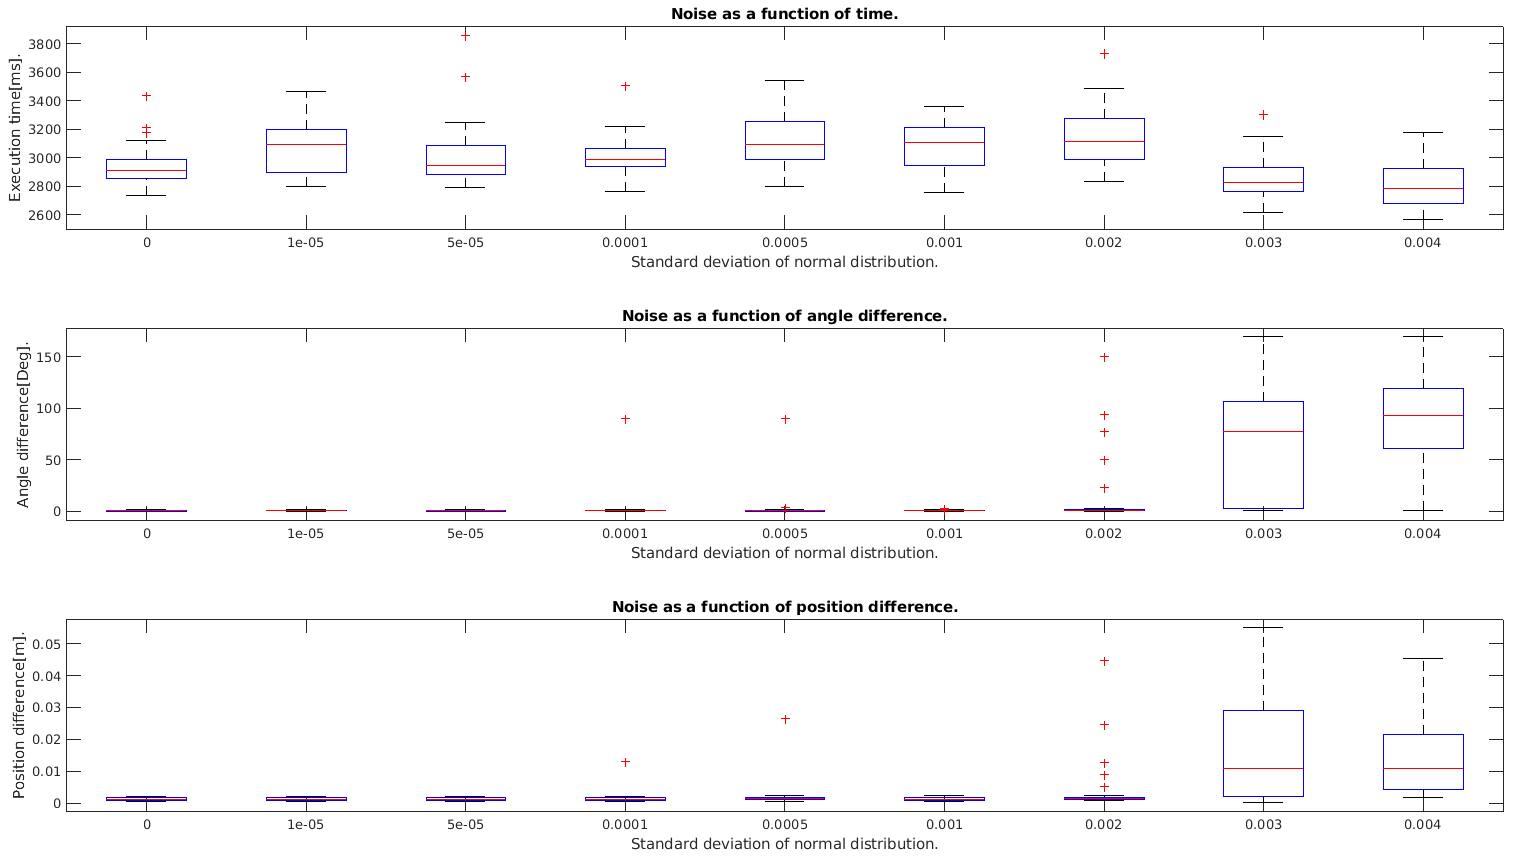
\includegraphics[width=1.1\textwidth]{figures/simulated_depth_sensor/noise_analysis.png}}
    \caption{Boxplot of the evaluation of method 2. The top figure shows the execution time versus the added noise. The middle figure shows the difference in angle versus the added noise. The bottom figure shows the difference in position versus the added noise.}
    \label{fig:method3_noise_analysis}
\end{figure}
From Figure \ref{fig:method3_noise_analysis}, it can be seen that the method performs acceptably until a noise with a standard deviation of $0.002$. The average execution time for which the method is deemed acceptable is $3.043(\pm 1.865)$ seconds, the average intrinsic notion distance is $1.708(\pm 9.380)$ degrees and the average euclidean distance between the real position and the estimated position is $0.0015 (\pm 0.00211)$ meter.

The implemented method has a limitation in the choice of object because validation of the alignment is based on the number of inliers. For example, if the object had been a box the number of inliers when the box is aligned on a table, would be high, thus the method would have a hard time estimation the true pose of the box. However, this was compensated by the use of a non-uniform object, a rubber duck \cite{rubber_duck} which can be seen in Figure \ref{fig:random_positions}.

\subsection{Method 3: Sparse Stereo} \label{subsec:method3}
Sparse stereo is used to find points in 3D space corresponding to sets of matched points on the object. The images are obtained with the two simulated cameras placed in the given workcell in RobWorks. Figure \ref{fig:sparse_stereo_pipeline} shows the steps for retrieving 3D points for a set of images.

\begin{figure}[H]
    \centering
    \noindent\makebox[\textwidth][c]{\subfile{figures/sparse_stereo/pipeline}}
    \caption{Illustration of the pipeline for the sparse stereo method.}
    \label{fig:sparse_stereo_pipeline}
\end{figure}

To make sure the object is isolated in the images the object is assumed to have a certain color. In this case, the object is red for a high contrast to the rest of the scene. This way, as seen in Figure \ref{subfig:filtered_duck}, the object can be isolated by filtering the color in the images. To find features in the images the Speeded-Up Robust Features, SURF, algorithm was implemented using OpenCV \cite{opencv}. The features matched are seen in Figure \ref{subfig:matched_duck}.

\begin{figure}[H]
    \centering
    \begin{subfigure}[t]{\textwidth}
        \centering
        \captionsetup{width=0.85\textwidth}
        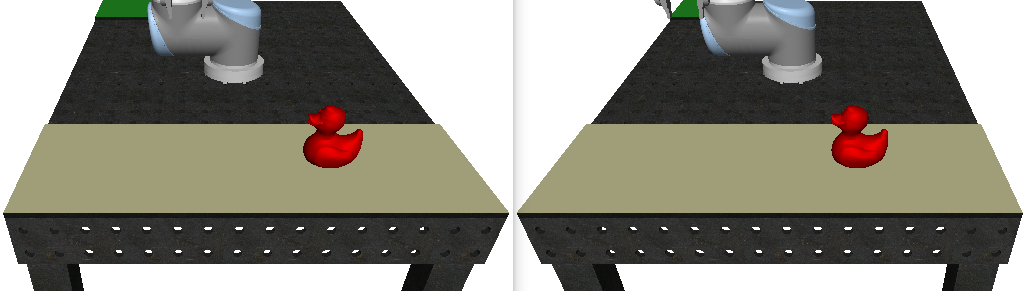
\includegraphics[width=0.85\textwidth]{figures/sparse_stereo/sparse_input_duck.png}
        \caption{Left and right image directly from the simulated cameras.}
        \label{subfig:left_right_input}
    \end{subfigure}
    
    \begin{subfigure}[t]{\textwidth}
        \centering
        \captionsetup{width=0.85\textwidth}
        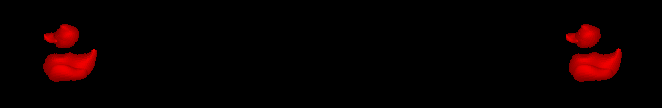
\includegraphics[width=0.85\textwidth]{figures/sparse_stereo/colour_filtered_duck.png}
        \caption{Left and right image after color filtering.}
        \label{subfig:filtered_duck}
    \end{subfigure}
    
    \begin{subfigure}[t]{\textwidth}
        \centering
        \captionsetup{width=0.85\textwidth}
        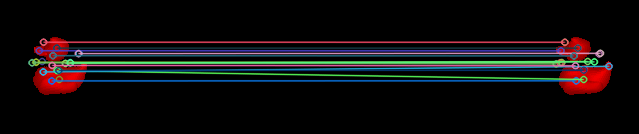
\includegraphics[width=0.85\textwidth]{figures/sparse_stereo/matched_points_duck.png}
        \caption{Left and right image with matched points.}
        \label{subfig:matched_duck}
    \end{subfigure}
    \caption{The process for finding matching points on the object.}
    \label{fig:my_label}
\end{figure}

After finding matched features in the two images, triangulation is used to find the estimated position in 3D space for each point. Then the average distance to all other points is calculated for each point, and the point with the lowest value is the point chosen to represent the detected object's position. With this method, the points found are on the surface of the object towards the cameras. Hence, it is not the most well suited for irregular shapes if desiring a complete pose estimation. For the rubber duck used in this example the default error between the detected point and center of the object changes with the orientation of the object.

\subsubsection{Evaluation of the Method} \label{subsubsec:eval_method3}
The robustness of the method is tested by adding Gaussian noise, with a mean of 0 and varying standard deviation, to the images. The standard deviation was tested from 0 to 25 in steps of 0.5. The random positions of the object are the same as in \ref{subsubsec:eval_method2}. The result is seen in Figure \ref{fig:sparse_noise}.

\begin{figure}[H]
    \centering
    \noindent\makebox[\textwidth]{%
    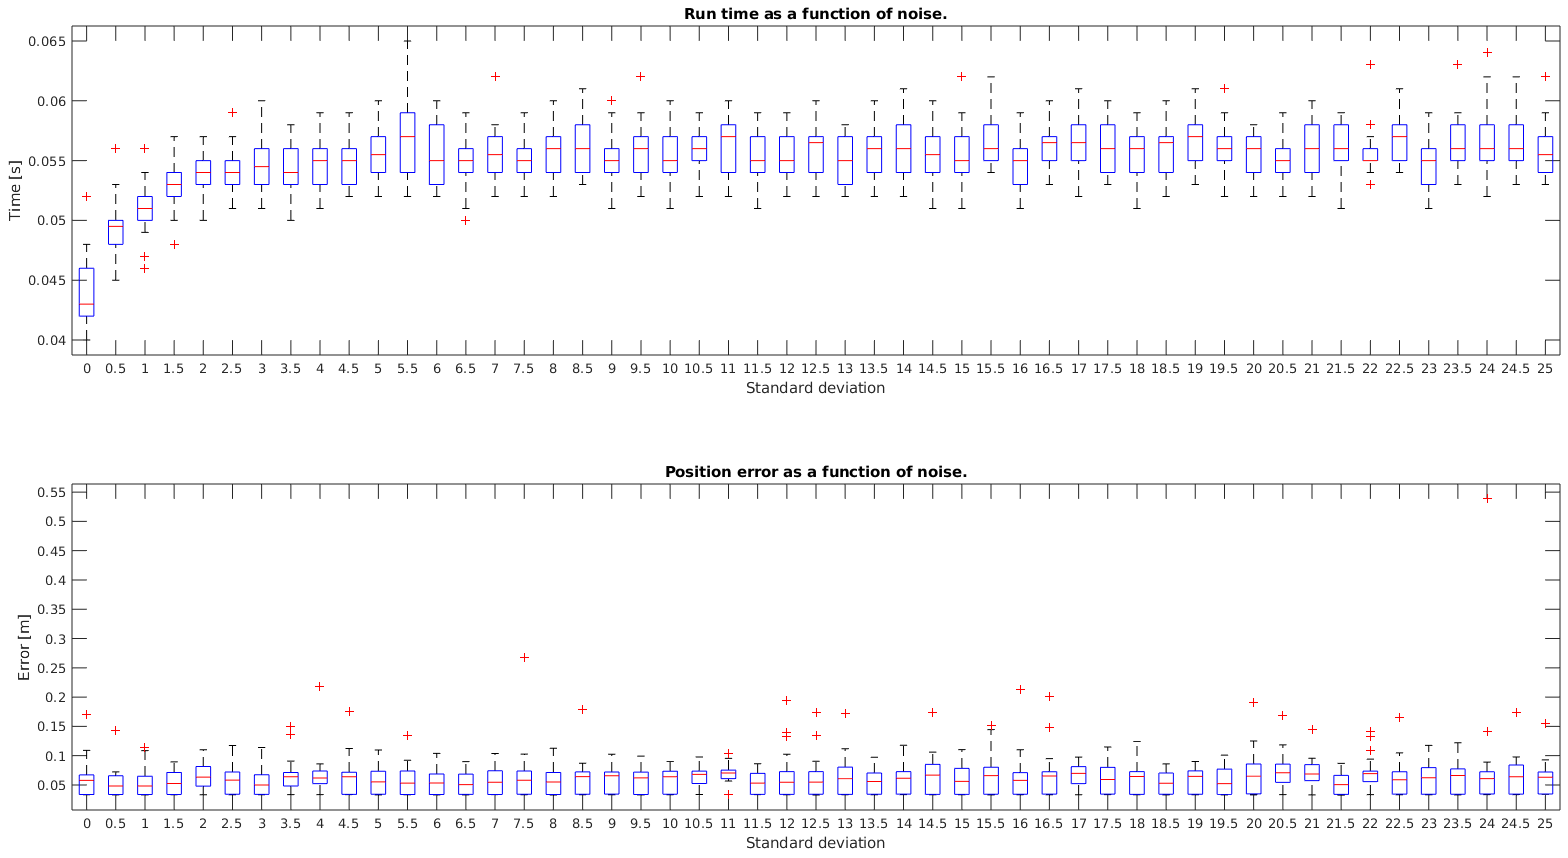
\includegraphics[width=1.2\textwidth]{figures/sparse_stereo/sparse_stereo_noise_test.png}}
    \caption{Execution time and error in estimated position with increasing levels of noise added to the picture.}
    \label{fig:sparse_noise}
\end{figure}

From Figure \ref{fig:sparse_noise}, it can be seen that the method is very robust and can manage noise from a normal distribution with a standard deviation of up to 25 without failing. However, the euclidean distance from the real position to the estimated position has an average error of $0.0552 (\pm 0.0029)$ meters and average execution time of $0.0606 (\pm 0.0287)$ seconds. The position error occurs because the found 3D point is on the surface of the duck, which has a non-uniform structure, and the real position is at the center of the duck. This method does therefore not suit non-uniform objects and would perform better if the object was uniform, e.g. a ball.

\subsection{Comparison of the Pose Estimation Methods Implemented} \label{subsec:vision_comparison}
To compare the two implemented pose estimation methods the execution time, the angle error between the real rotation and the estimated rotation and the euclidean distance between the real position and the estimated position are considered. Furthermore, the robustness of the method is also considered, meaning how much noise from a normal distribution the method can tolerate. Table \ref{tab:vision_comp} shows a summary of the results of the pose estimation methods.

\begin{table}[H]
\centering
\resizebox{\textwidth}{!}{%
\begin{tabular}{lcc}
\toprule
& \textbf{Method 2: Simulated depth sensor} & \textbf{Method 3: Sparse stereo} \\ \midrule
\textbf{Robustness [std. deviation]} & 0.001 & 25 \\
\textbf{Execution time [s]} & $3.043(\pm 1.865)$ & $0.0606 (\pm 0.0287)$ \\
\textbf{Rotation error [Deg]} & $1.708 (\pm 9.380)$ & $\div$ \\
\textbf{Position error [m]} & $0.0015 (\pm 0.00211)$ & $0.0552(\pm 0.0029)$ \\ \bottomrule
\end{tabular}%
}
\caption{Summary of the implemented pose estimation methods.}
\label{tab:vision_comp}
\end{table}

Table \ref{tab:vision_comp} shows the strengths and weaknesses of the two pose estimation methods. 

The simulated depth sensor method has a small position error and angle error. However, it can only tolerate noise from a normal distribution with a standard deviation of max 0.001, and the execution time is higher than the sparse stereo method.

The sparse stereo method does not calculate a rotation, thus if the object to grasp has to be grasped from a certain angle this method would not work. The sparse stereo method would work well for a uniform object, such as a ball. Furthermore, the method can sustain more noise than the simulated depth sensor method.

Thus, the sparse stereo method would be chosen for simple uniform objects and the simulated depth sensor method for non-uniform objects.

\end{document}